
\begin{figure*}[ht]
  \centering
  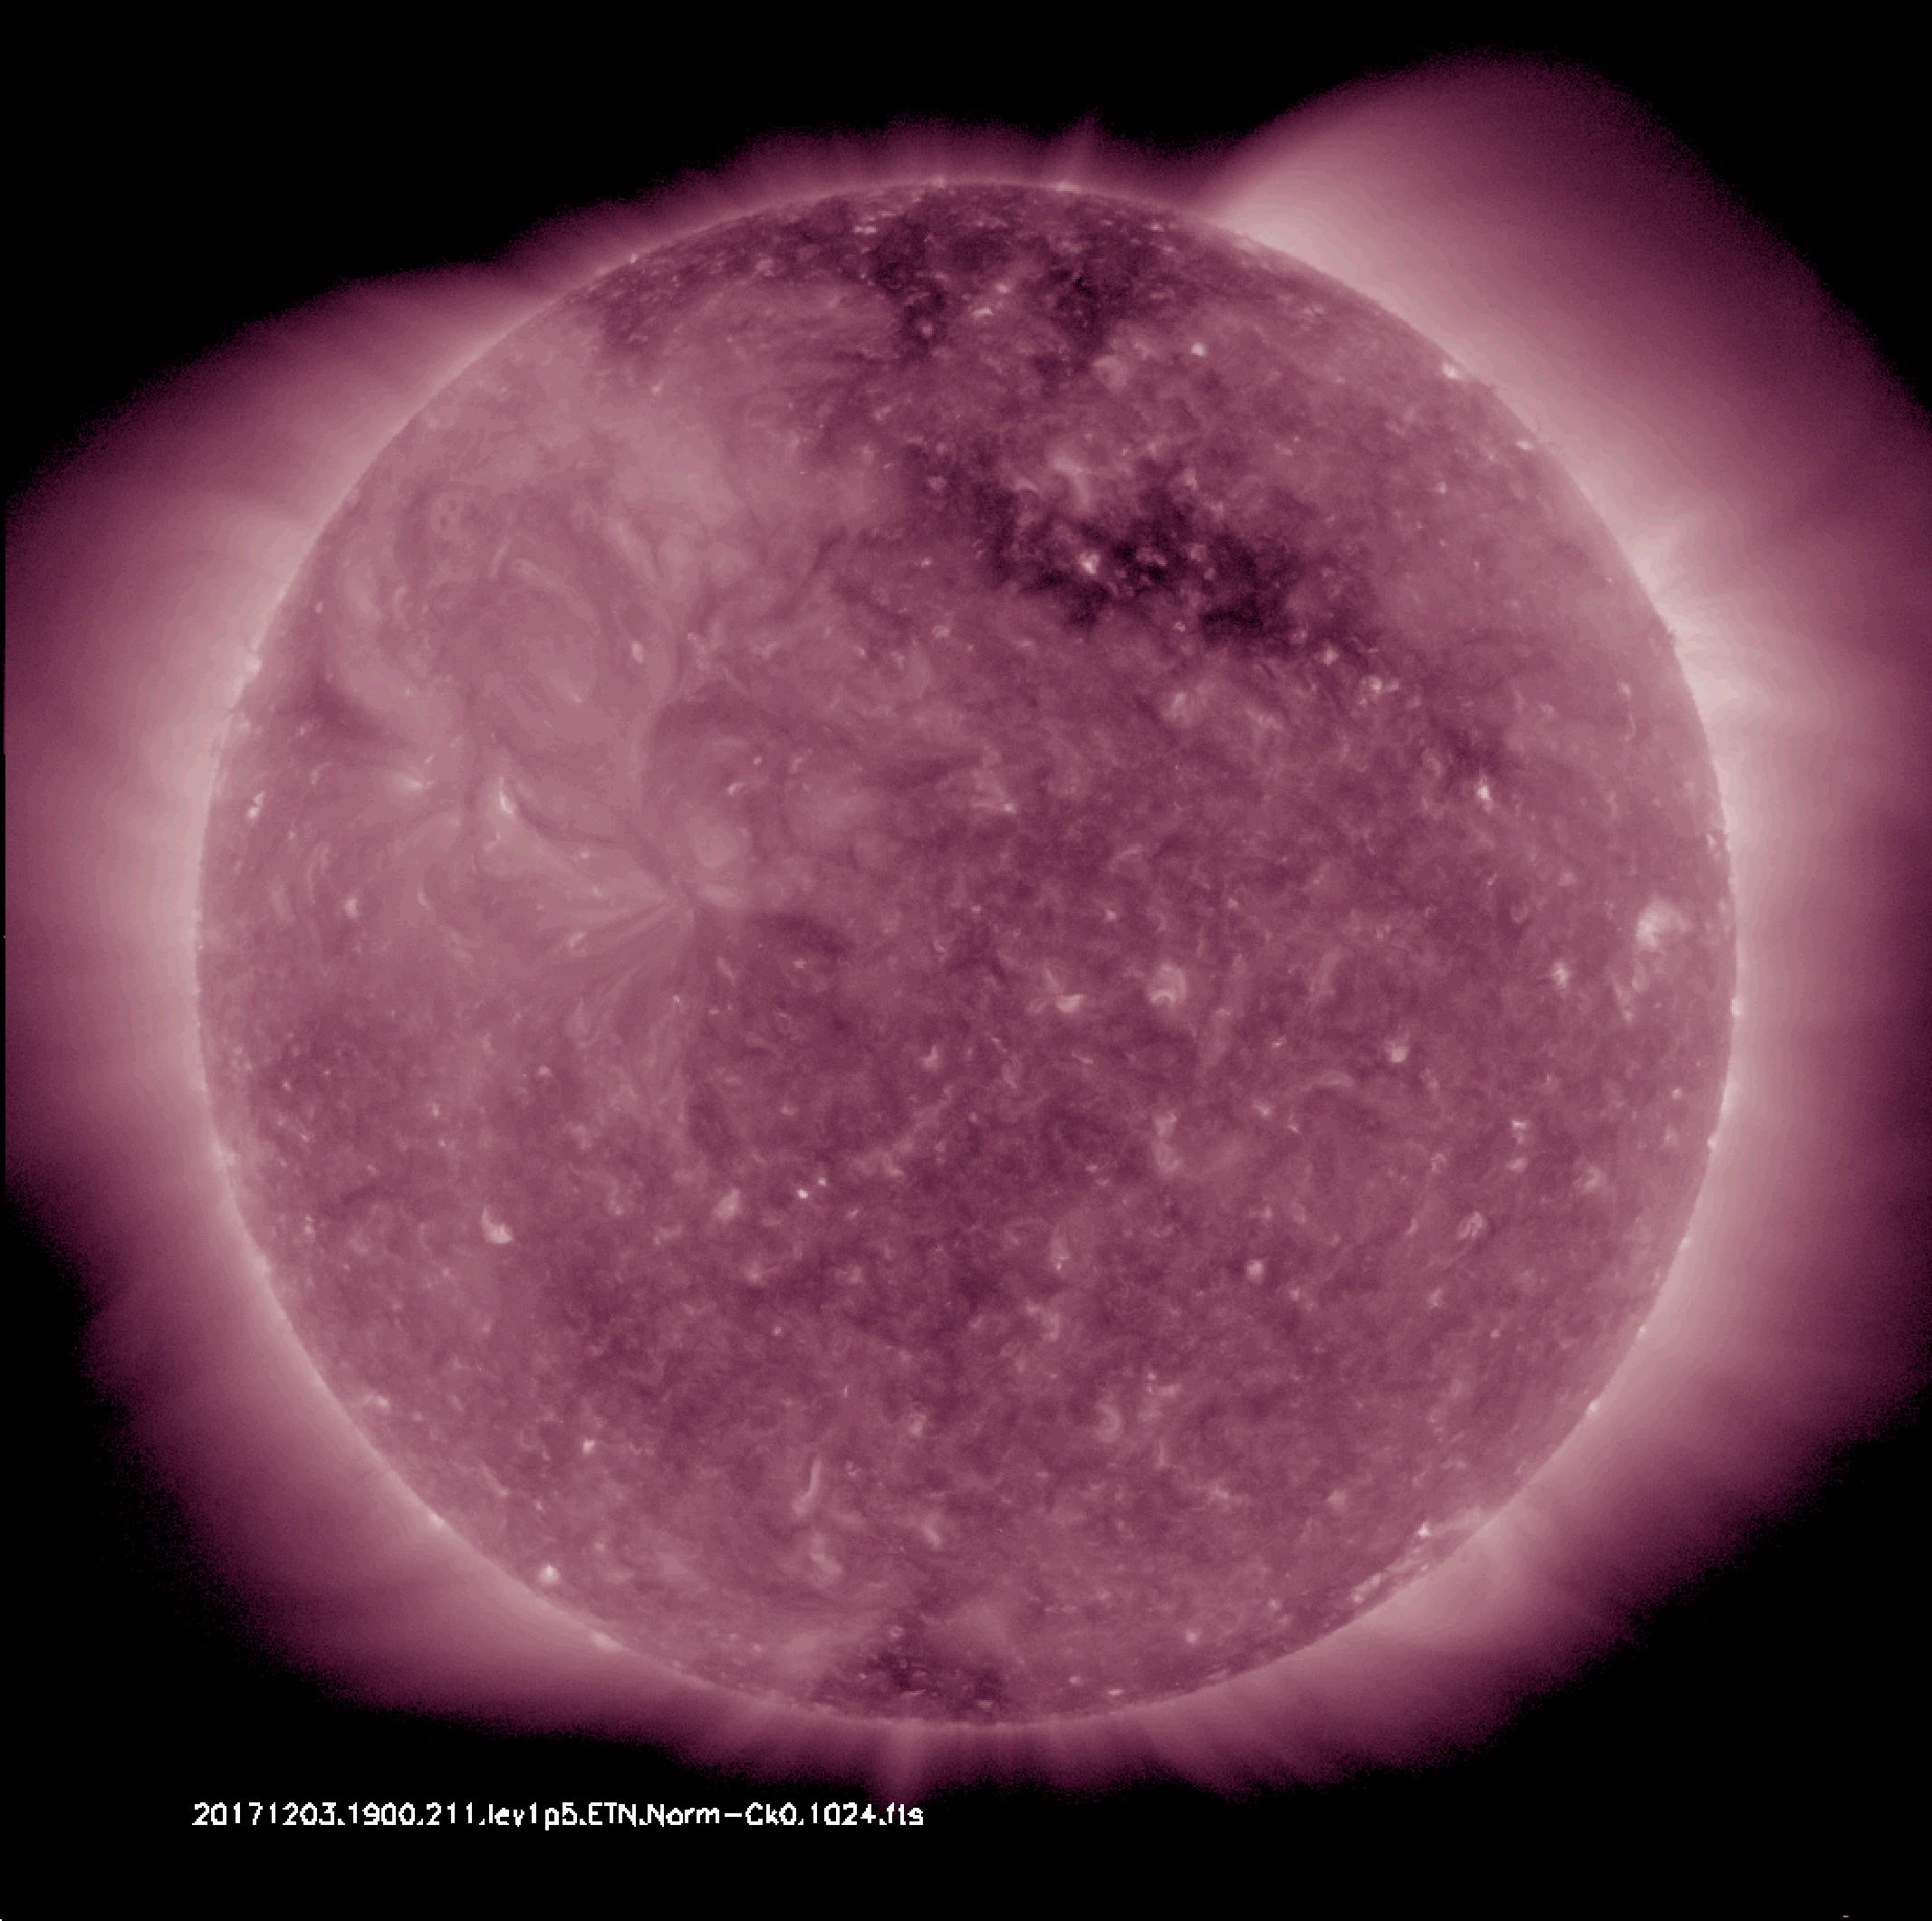
\includegraphics[width=0.67\columnwidth]{img_211.pdf}
  \hskip 1.5cm
  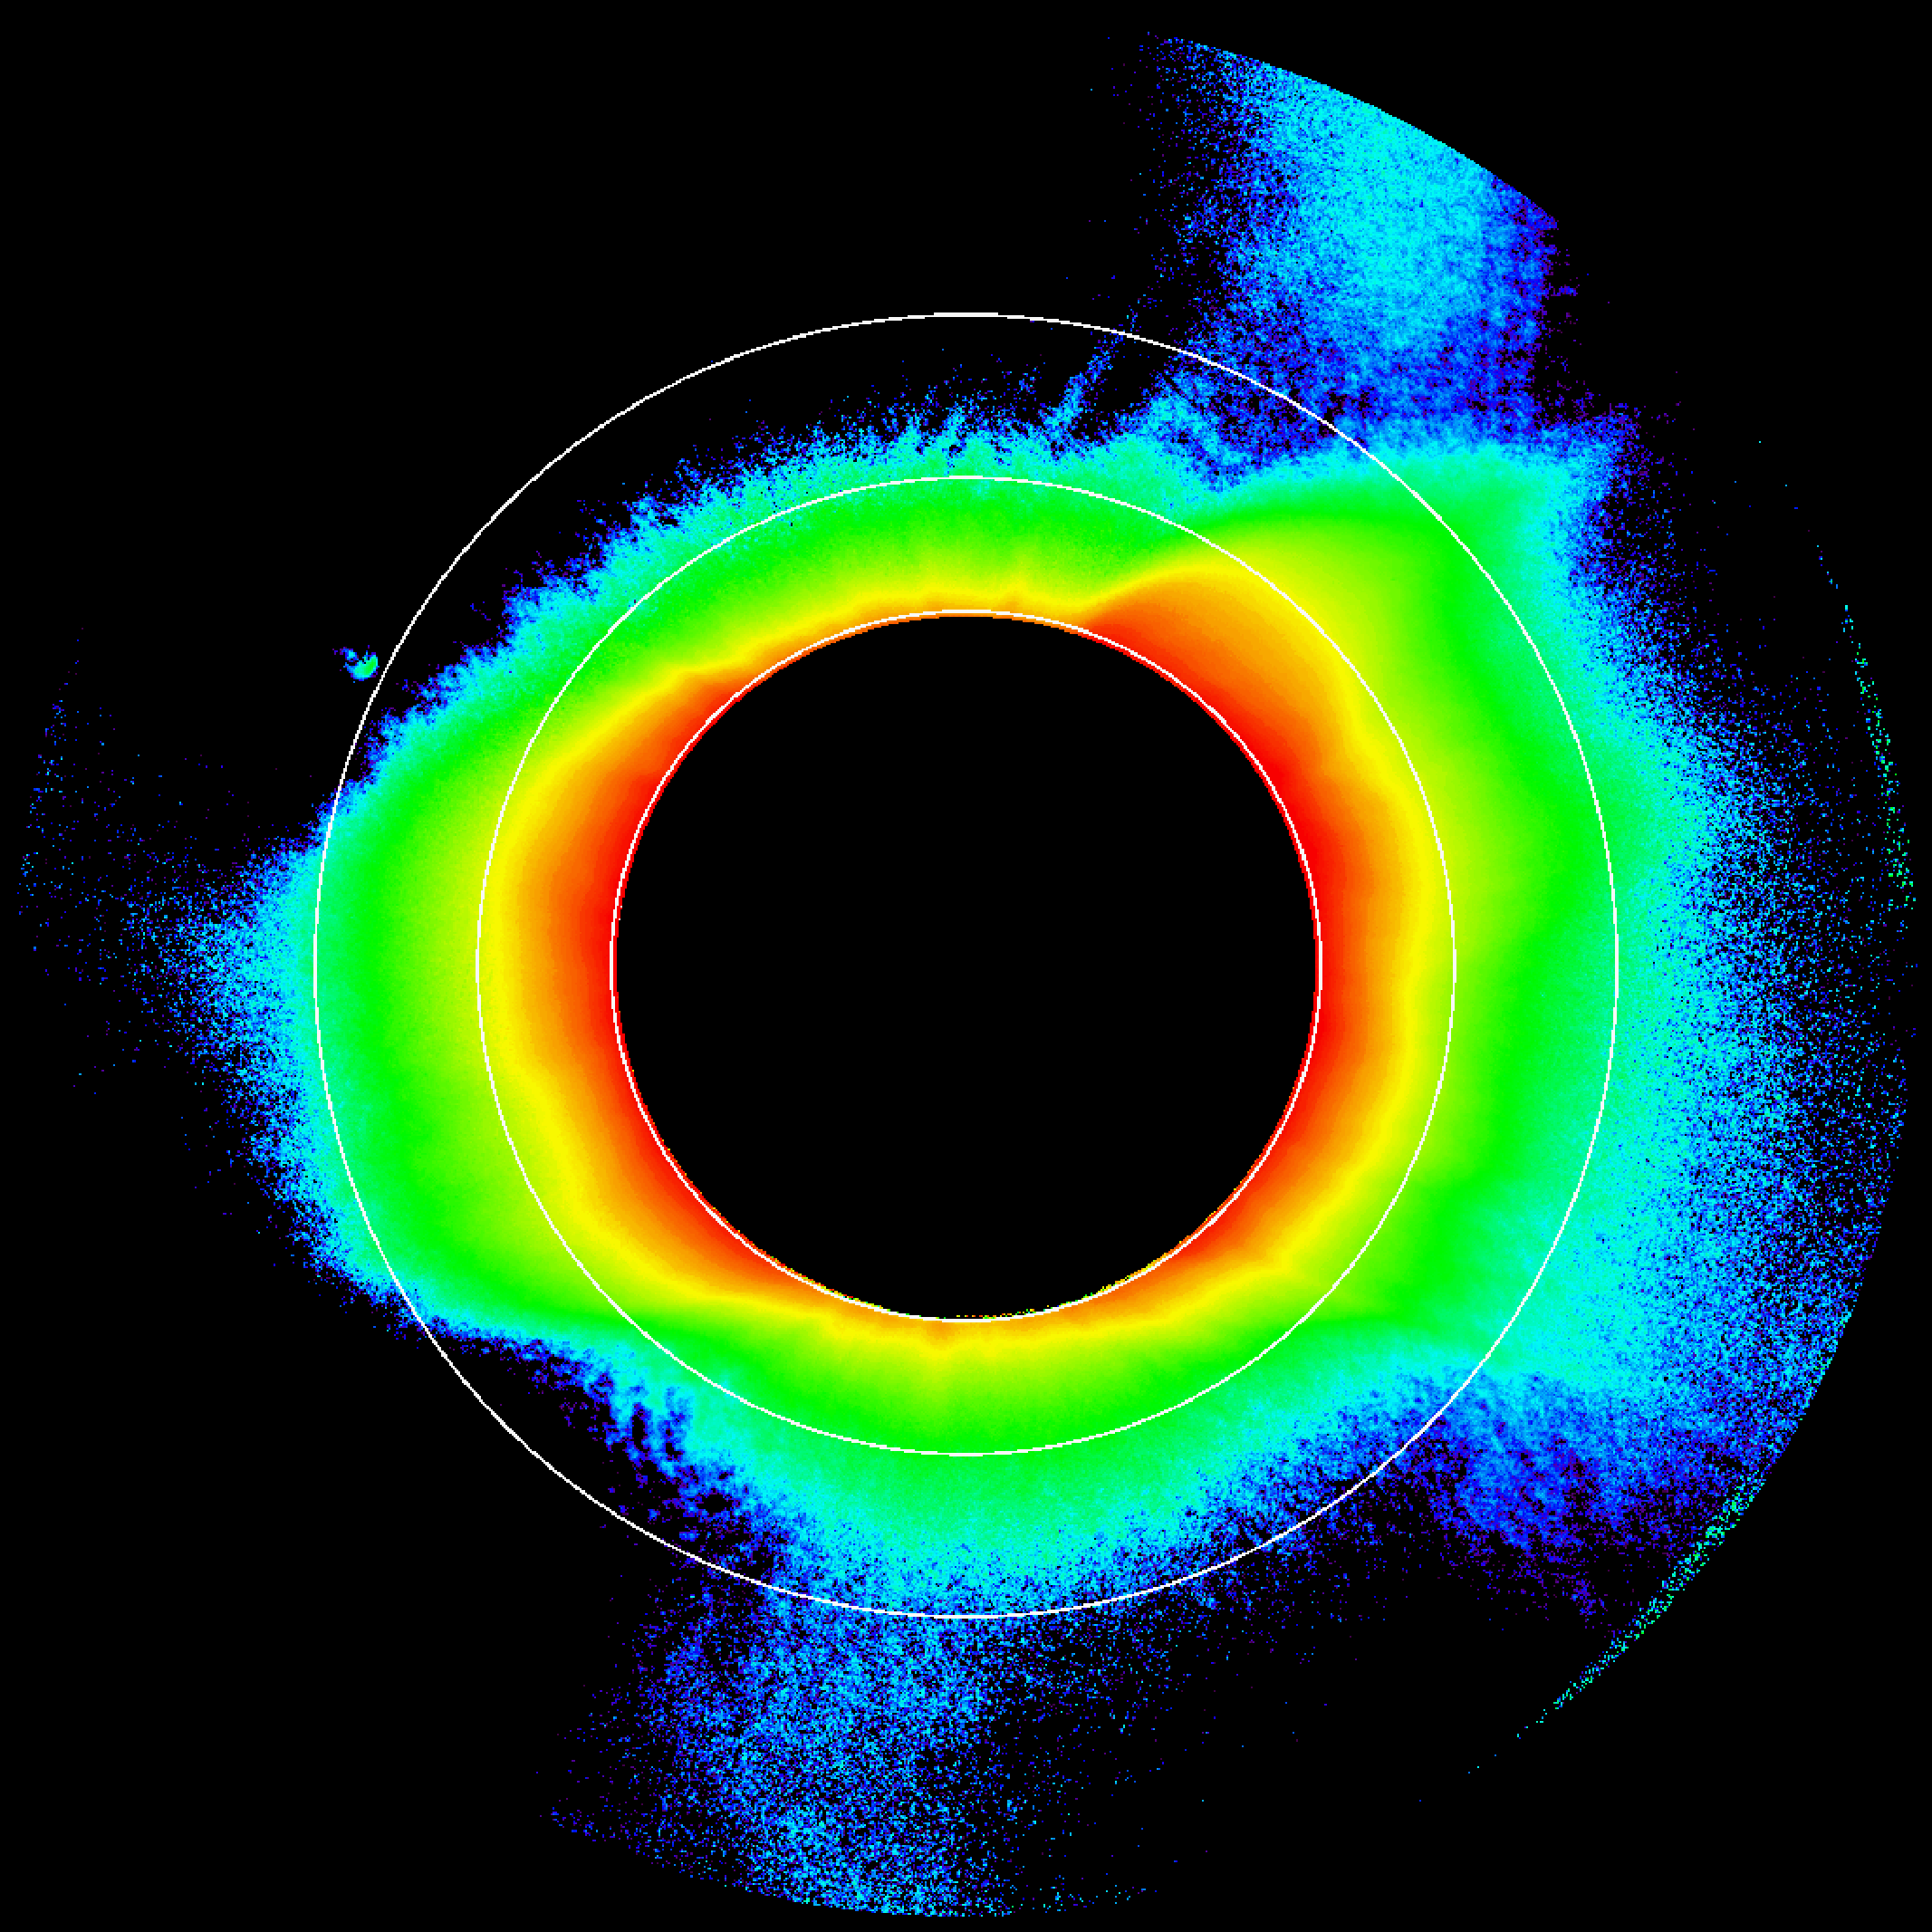
\includegraphics[width=0.67\columnwidth]{20171203_180316_kcor_l1_10min_avg_image.pdf}
  \caption{Example of images used for tomographic reconstruction of the coronal electron density of CR-2198 (see text), both corresponding to 2017 December 03 UT 18:00-19:00. Left panel: SDO/AIA coronal EUV image in the $211~\rm{\AA}$ band. Right panel: HAO/KCOR coronal pB image, with white rings indicating heliocentric heights $1.09, 1.50, \rm{and}\, 2.0~\rm{R}_\odot$.}
  \label{fig_images}
\end{figure*}


\begin{figure*}[]
  \centering
  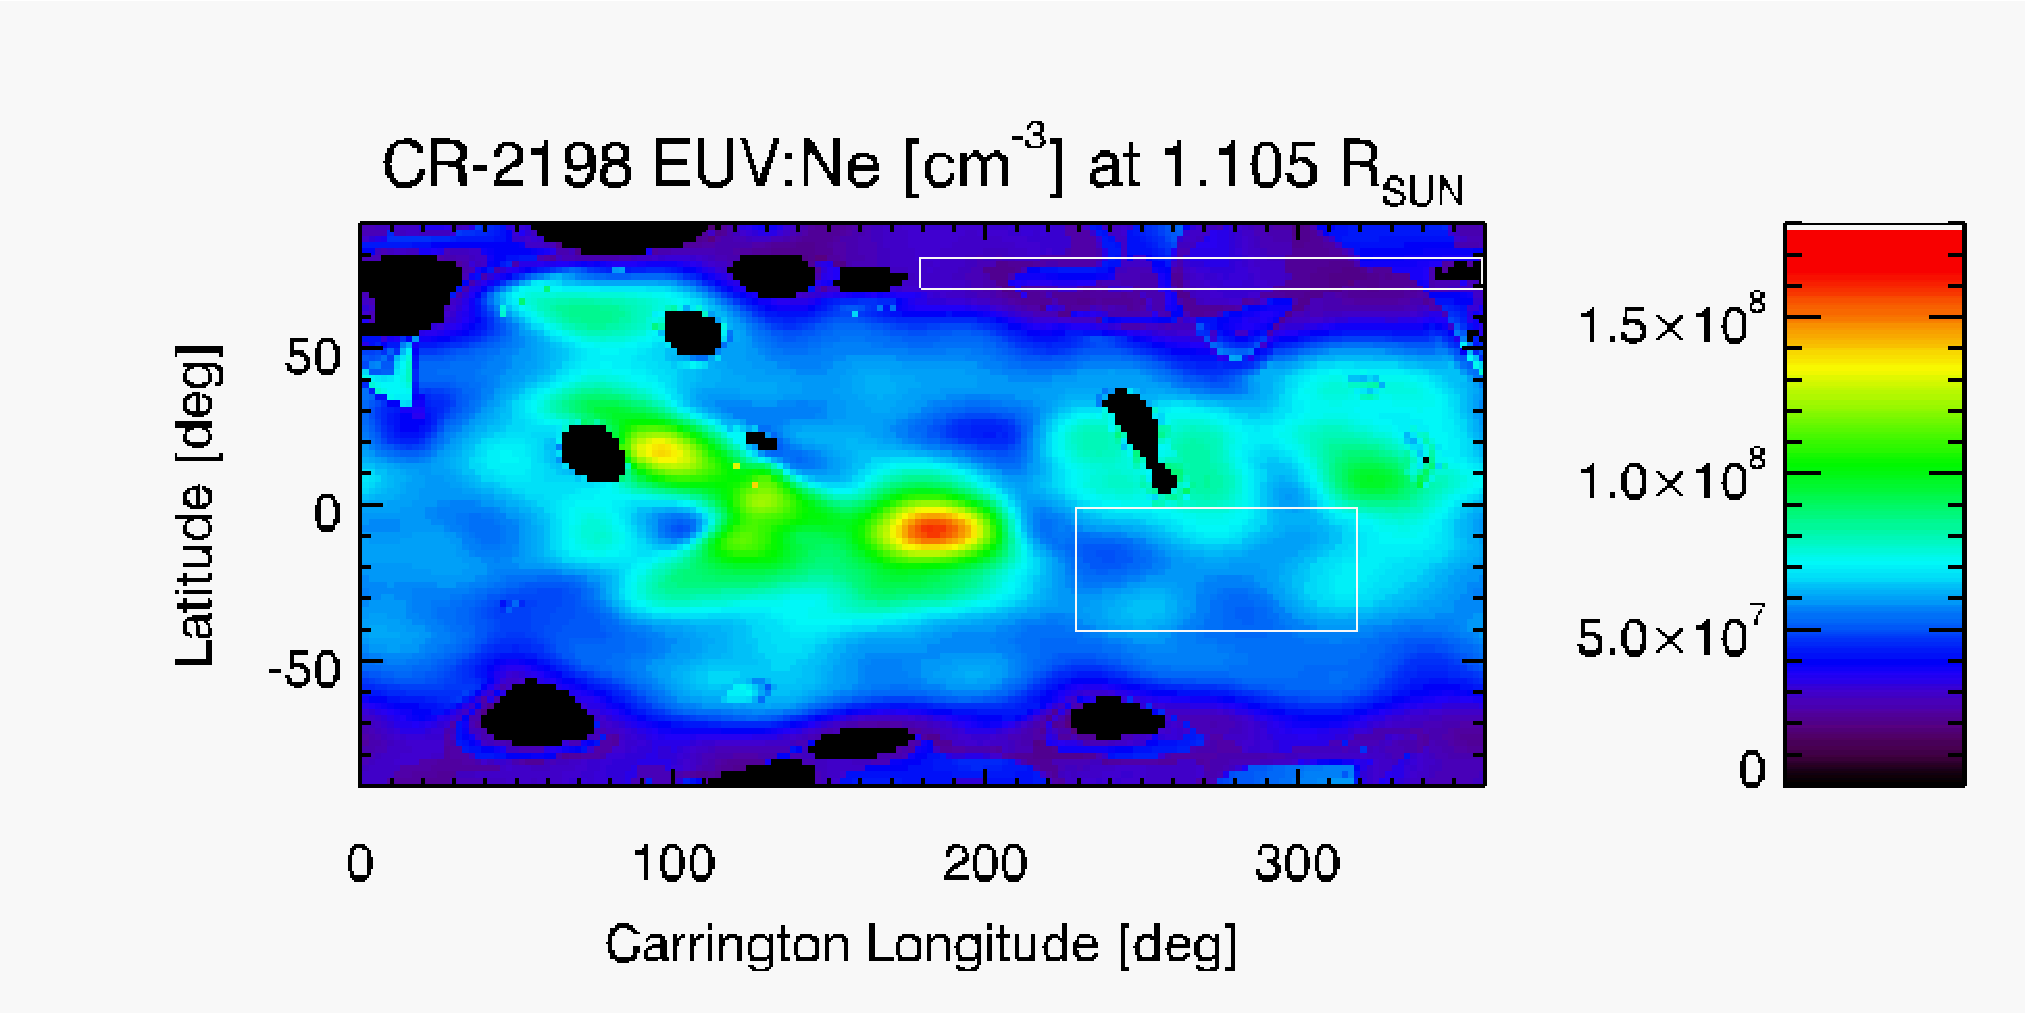
\includegraphics[width=\columnwidth]{map_Ne_CR2198_DEMT-AIA_H1-L799_r3D_reduced_1105_Rsun.pdf}
  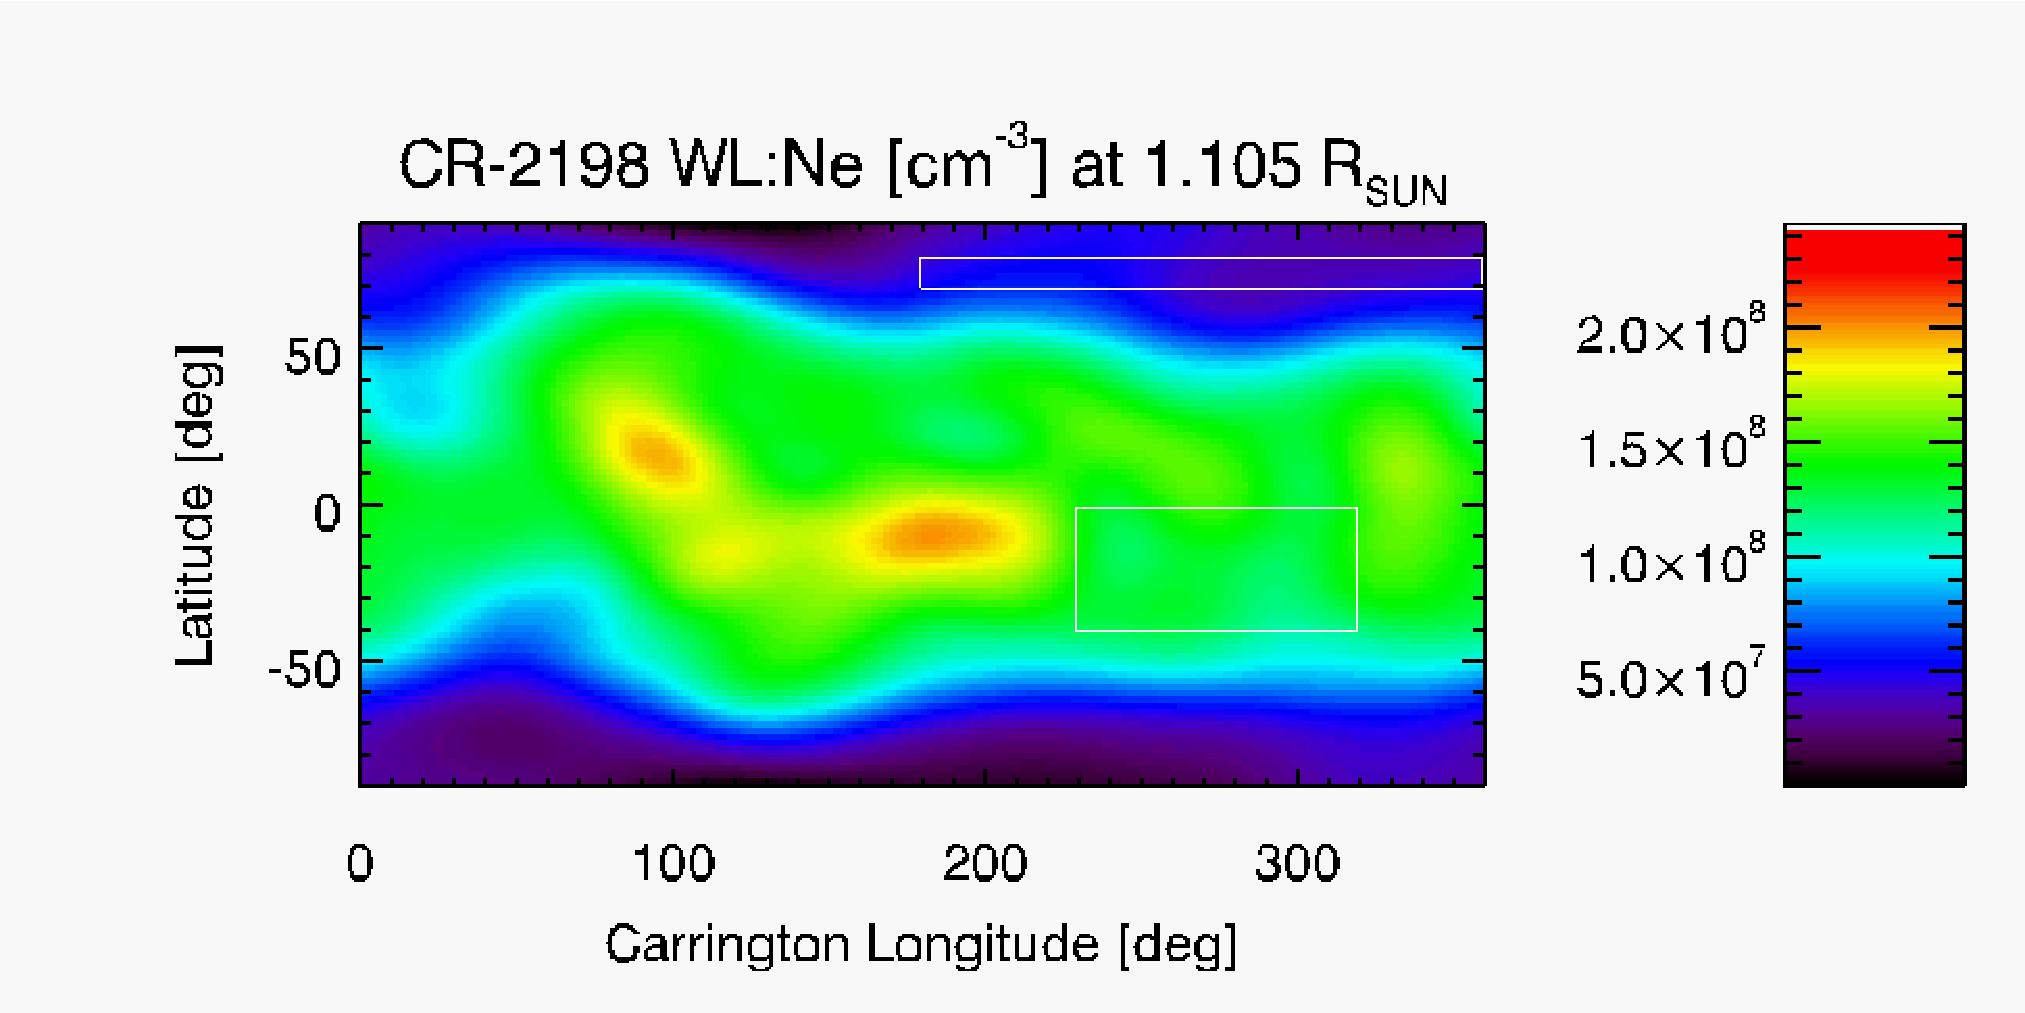
\includegraphics[width=\columnwidth]{map_x_KCORCR219813imgs-reducedbf2ri105ro225_Inst_109_200_120_90_180_dropneg_r3D_l1e-4_1105_Rsun.pdf}
  \caption{CR-2198: Same as Fig. \ref{fig_maps} but with the left panel showing the DEMT reconstruction based on EUV images blocked at projected radius $r<1.09~\rm{R}_\odot$, using 1 image per day. Regularization level of DEMT is optimal here.}
  \label{fig_maps6}
\end{figure*}

\begin{figure*}[!h]
  \centering
  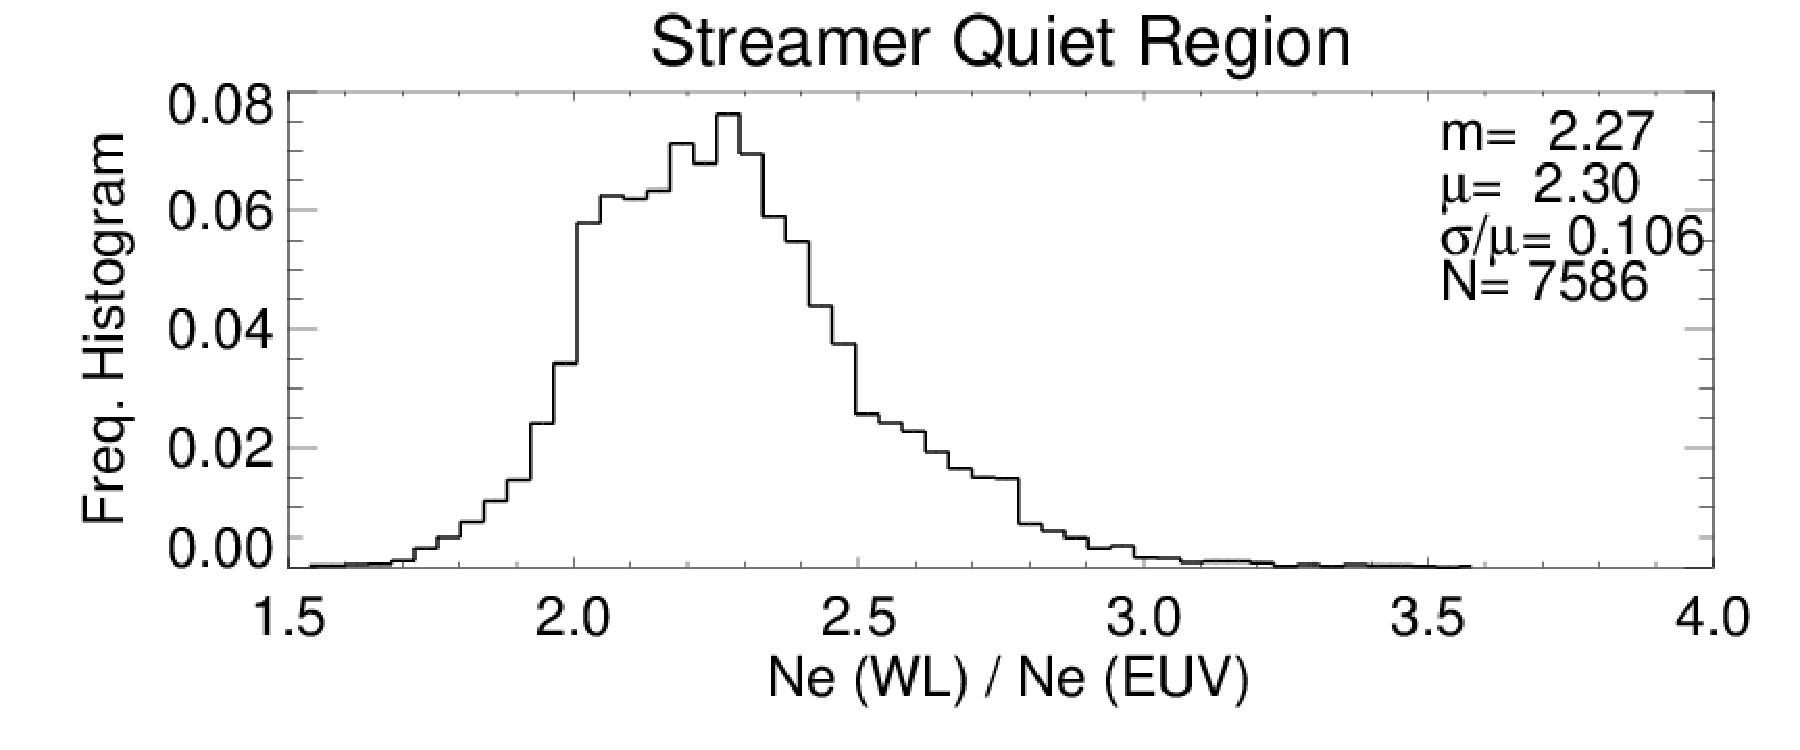
\includegraphics[width=\columnwidth]{comparison_KCOR-Tom_vs_DEMT_CR2198_h_l799_reduced_kcor_1e4_newgrid-Quiet-region1_ratio_range1105-1195_Rsun.pdf}
  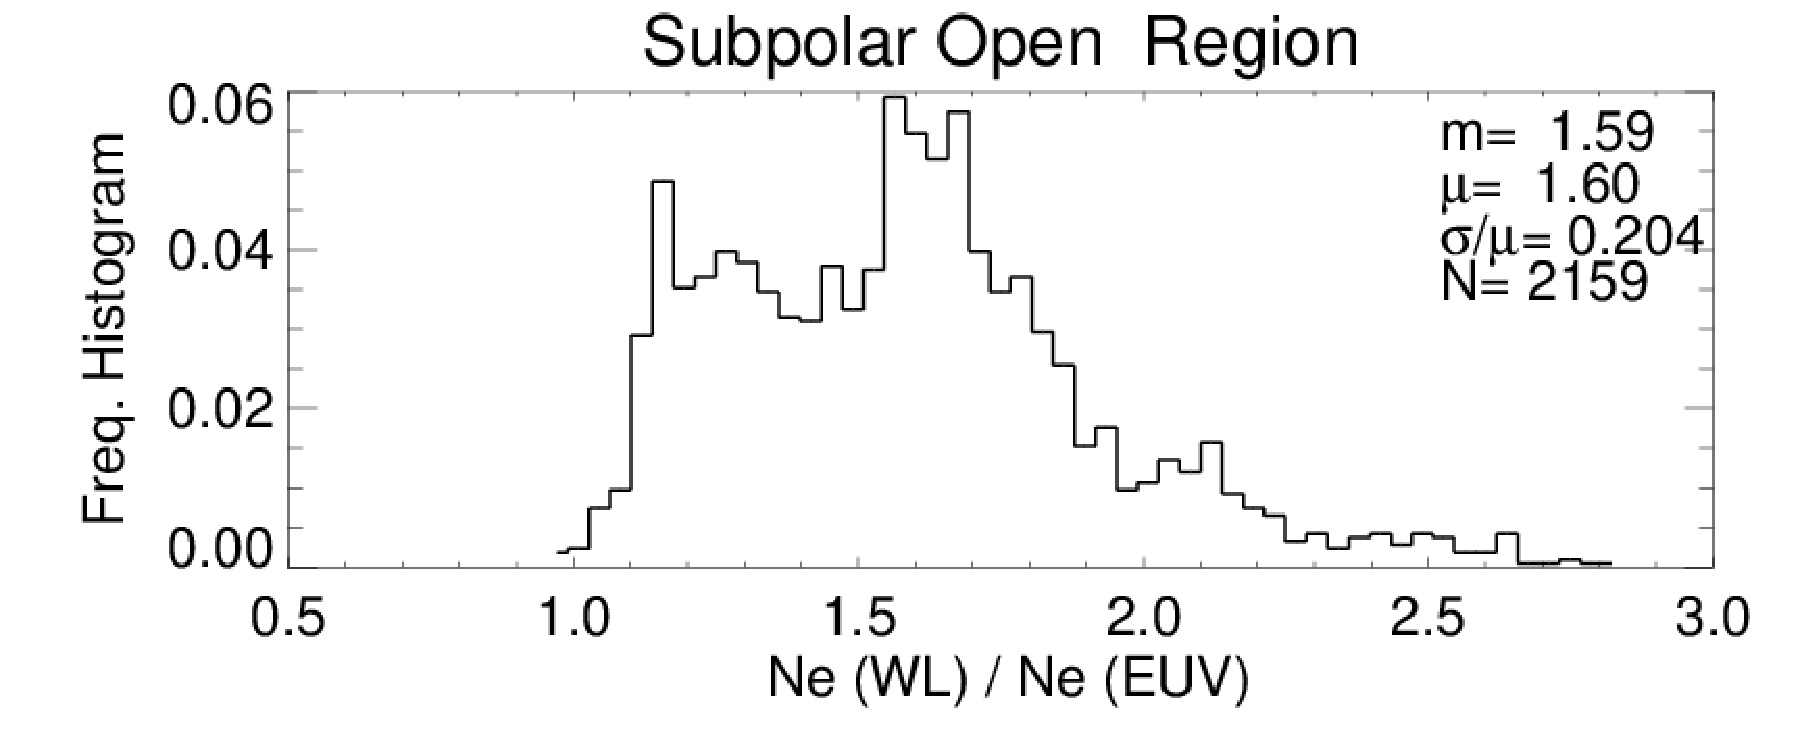
\includegraphics[width=\columnwidth]{comparison_KCOR-Tom_vs_DEMT_CR2198_h_l799_reduced_kcor_1e4_newgrid-Open-region_N_ratio_range1105-1155_Rsun.pdf}\\
  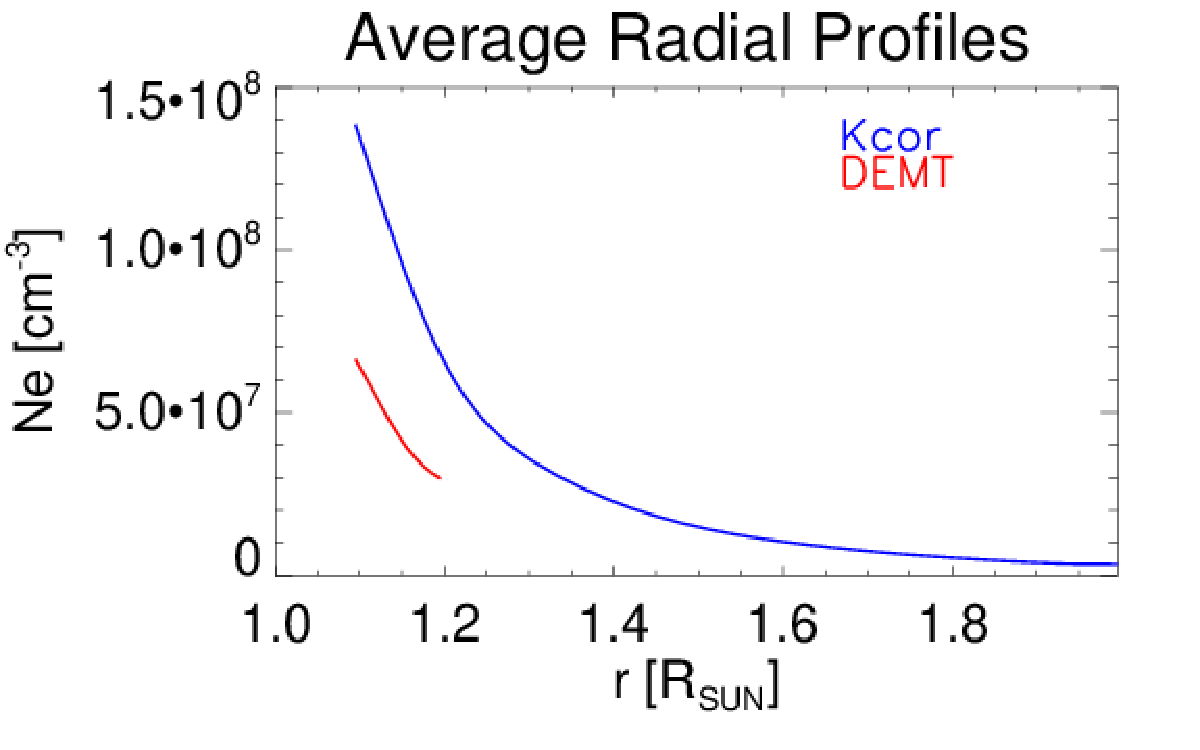
\includegraphics[width=0.75\columnwidth]{Average_Radial_Profiles_KCOR-Tom_vs_DEMT_CR2198_h_l799_reduced_kcor_1e4_newgrid-Quiet-region1.pdf}
  \hskip 2cm
  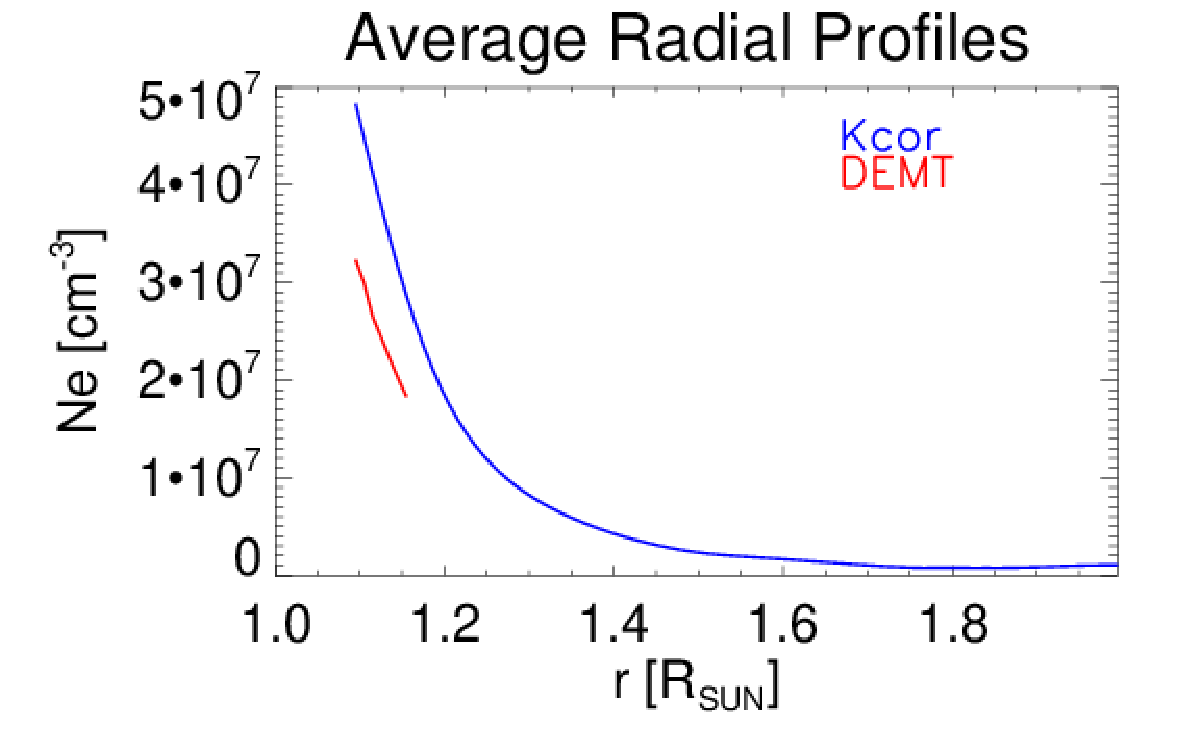
\includegraphics[width=0.75\columnwidth]{Average_Radial_Profiles_KCOR-Tom_vs_DEMT_CR2198_h_l799_reduced_kcor_1e4_newgrid-Open-region_N.pdf}
  \caption{Same analysis of Figure \ref{fig_analysis}, but for the reconstructions shown in Figure \ref{fig_maps6} above.}
  \label{fig_analysis6}
\end{figure*}
